In section 2.2.1 categories of medical smart phone apps were defined. Apps in the same categories might have a similar feature set and capabilities. An app in the \textit{Alert / First Response} category might have a database that stores important contacts in the user’s area and a user interface that allows the user to quickly alert a contact in an emergency situation. An app in the \textit{Learning / Educational / Reference} category might be modelled as a quiz app which presents the user with a question and several possible answers to choose from. Answers from several questions will can be evaluated and a score is presented to the user at the end of a session. The app would be implemented with a database of questions and weighted answers, as well as an interface that presents the questions to the user sequentially.

One of the goals of this project is to define requirements for an app that provides a risk assessment of a lesion being benign or malignant. A high level description of the primary function of the app is the following:

\begin{itemize}[label={}]
\item The smart phone app allows the user to capture and analyse an image of a skin lesion and provide a risk assessment to the user of the lesion being a malignant melanoma.

\end{itemize}

The user might also like to save the image and results in oder to be able to compare it with other assessments in the future, or to review the assessment with a dermatologist. For comparison it might be useful to save associated metadata, such as the date and location on the body of the lesion. For convenience it might be nice to send the assessment and image via email to a specialist for review.
Secondary functionality can be described as follows:

\begin{itemize}[label={}]
\item The app allows the user to save or archive the image and corresponding assessment for future comparison and review.
\item The user can add, edit, and save metadata associated with the image of the lesion.
\item The user can browse archived images, assessments, and associated metadata.
\item The user can send a set of images with associated assessment and metadata via email.
\end{itemize}

From this high level description some basic assumptions about the app’s architecture can already be made. The app will require access to a database that can store information about an image, results of the analysis, and metadata. The app will require a user interface that allows a user to browse and edit data associated with an image. The app requires access to the smart phone’s camera api in order to capture images.
Another consideration that will impact design decisions is the investment already made in developing the image processing and analysis algorithms. Choosing python as the basis for the numerical algorithms and leveraging python based scientific computing libraries has implications because python code is not easily portable to iOS or Android devices. In order to efficiently utilise the algorithms as they are, and to continue to update and improve them, the image processing and analysis algorithms should be implemented as online services.

\begin{itemize}[label={}]
\item The image processing and risk assessment algorithms will be implemented as online services.
\end{itemize}

In order to formally elicit the requirements the hight level description will be broken down into structured use cases. A set of requirements will be extracted from the use cases.



\section{User Interface}
\begin{figure}[H]
\centering
    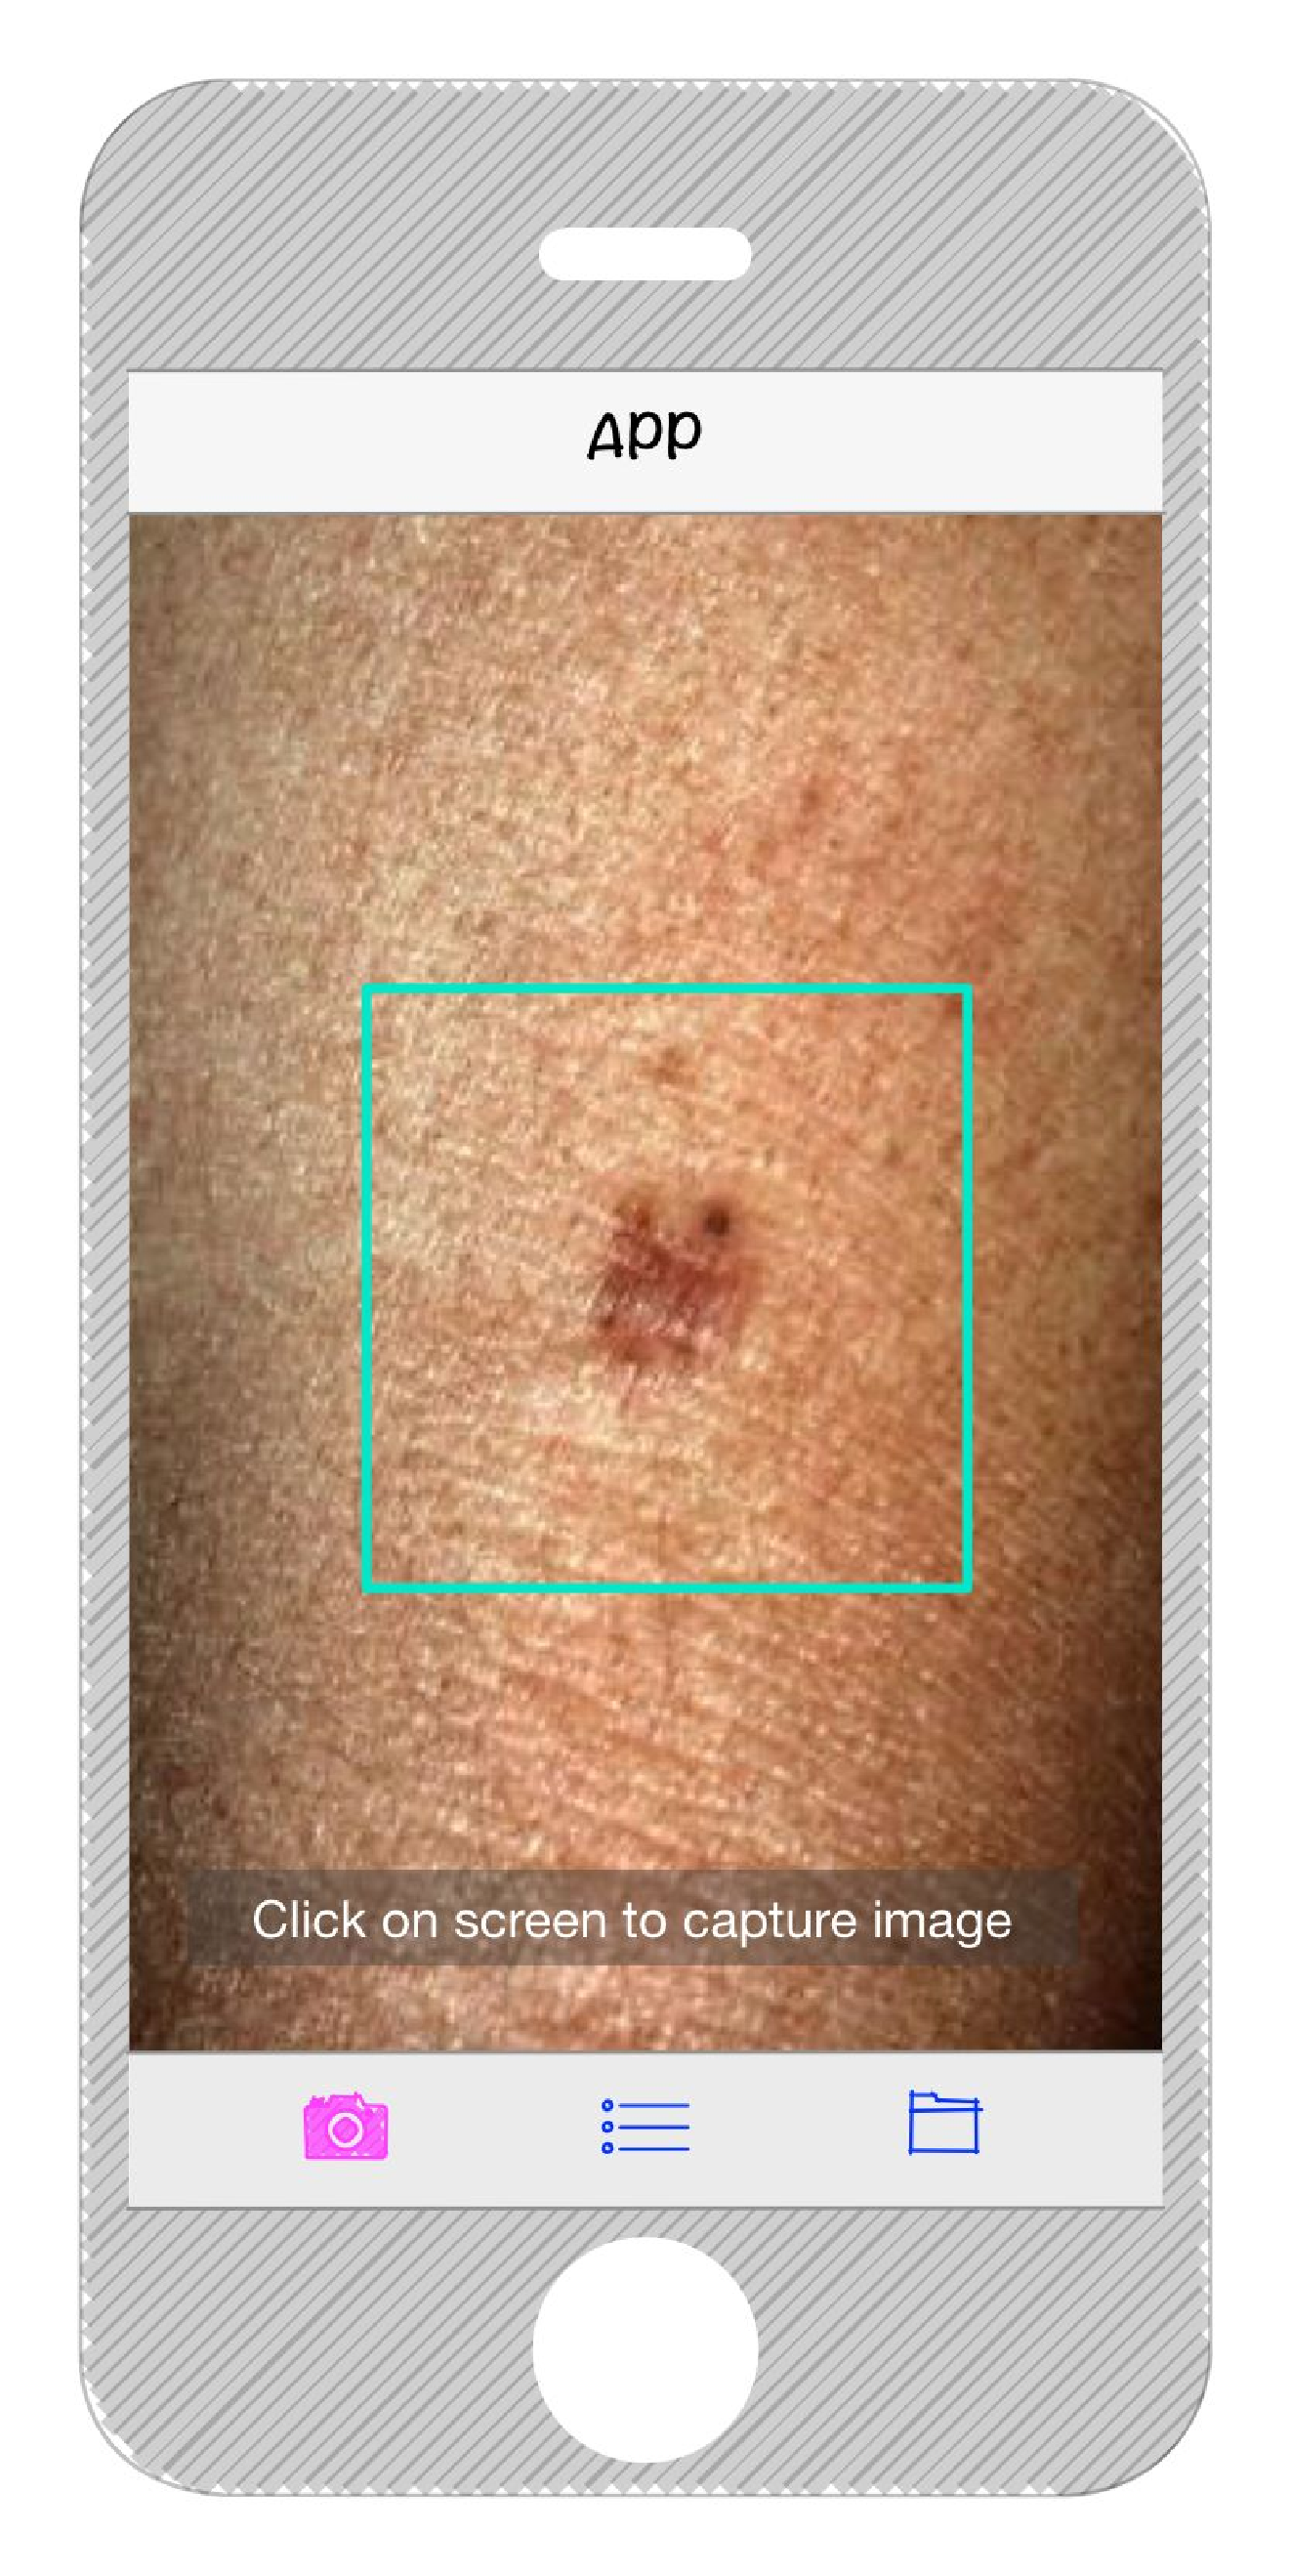
\includegraphics[height=10cm,keepaspectratio]{assets/GUI/image_capture.pdf}
    \caption{Image Capture View}
    \label{fig:image_capture}
\end{figure}

\begin{figure}[H]
    \centering
    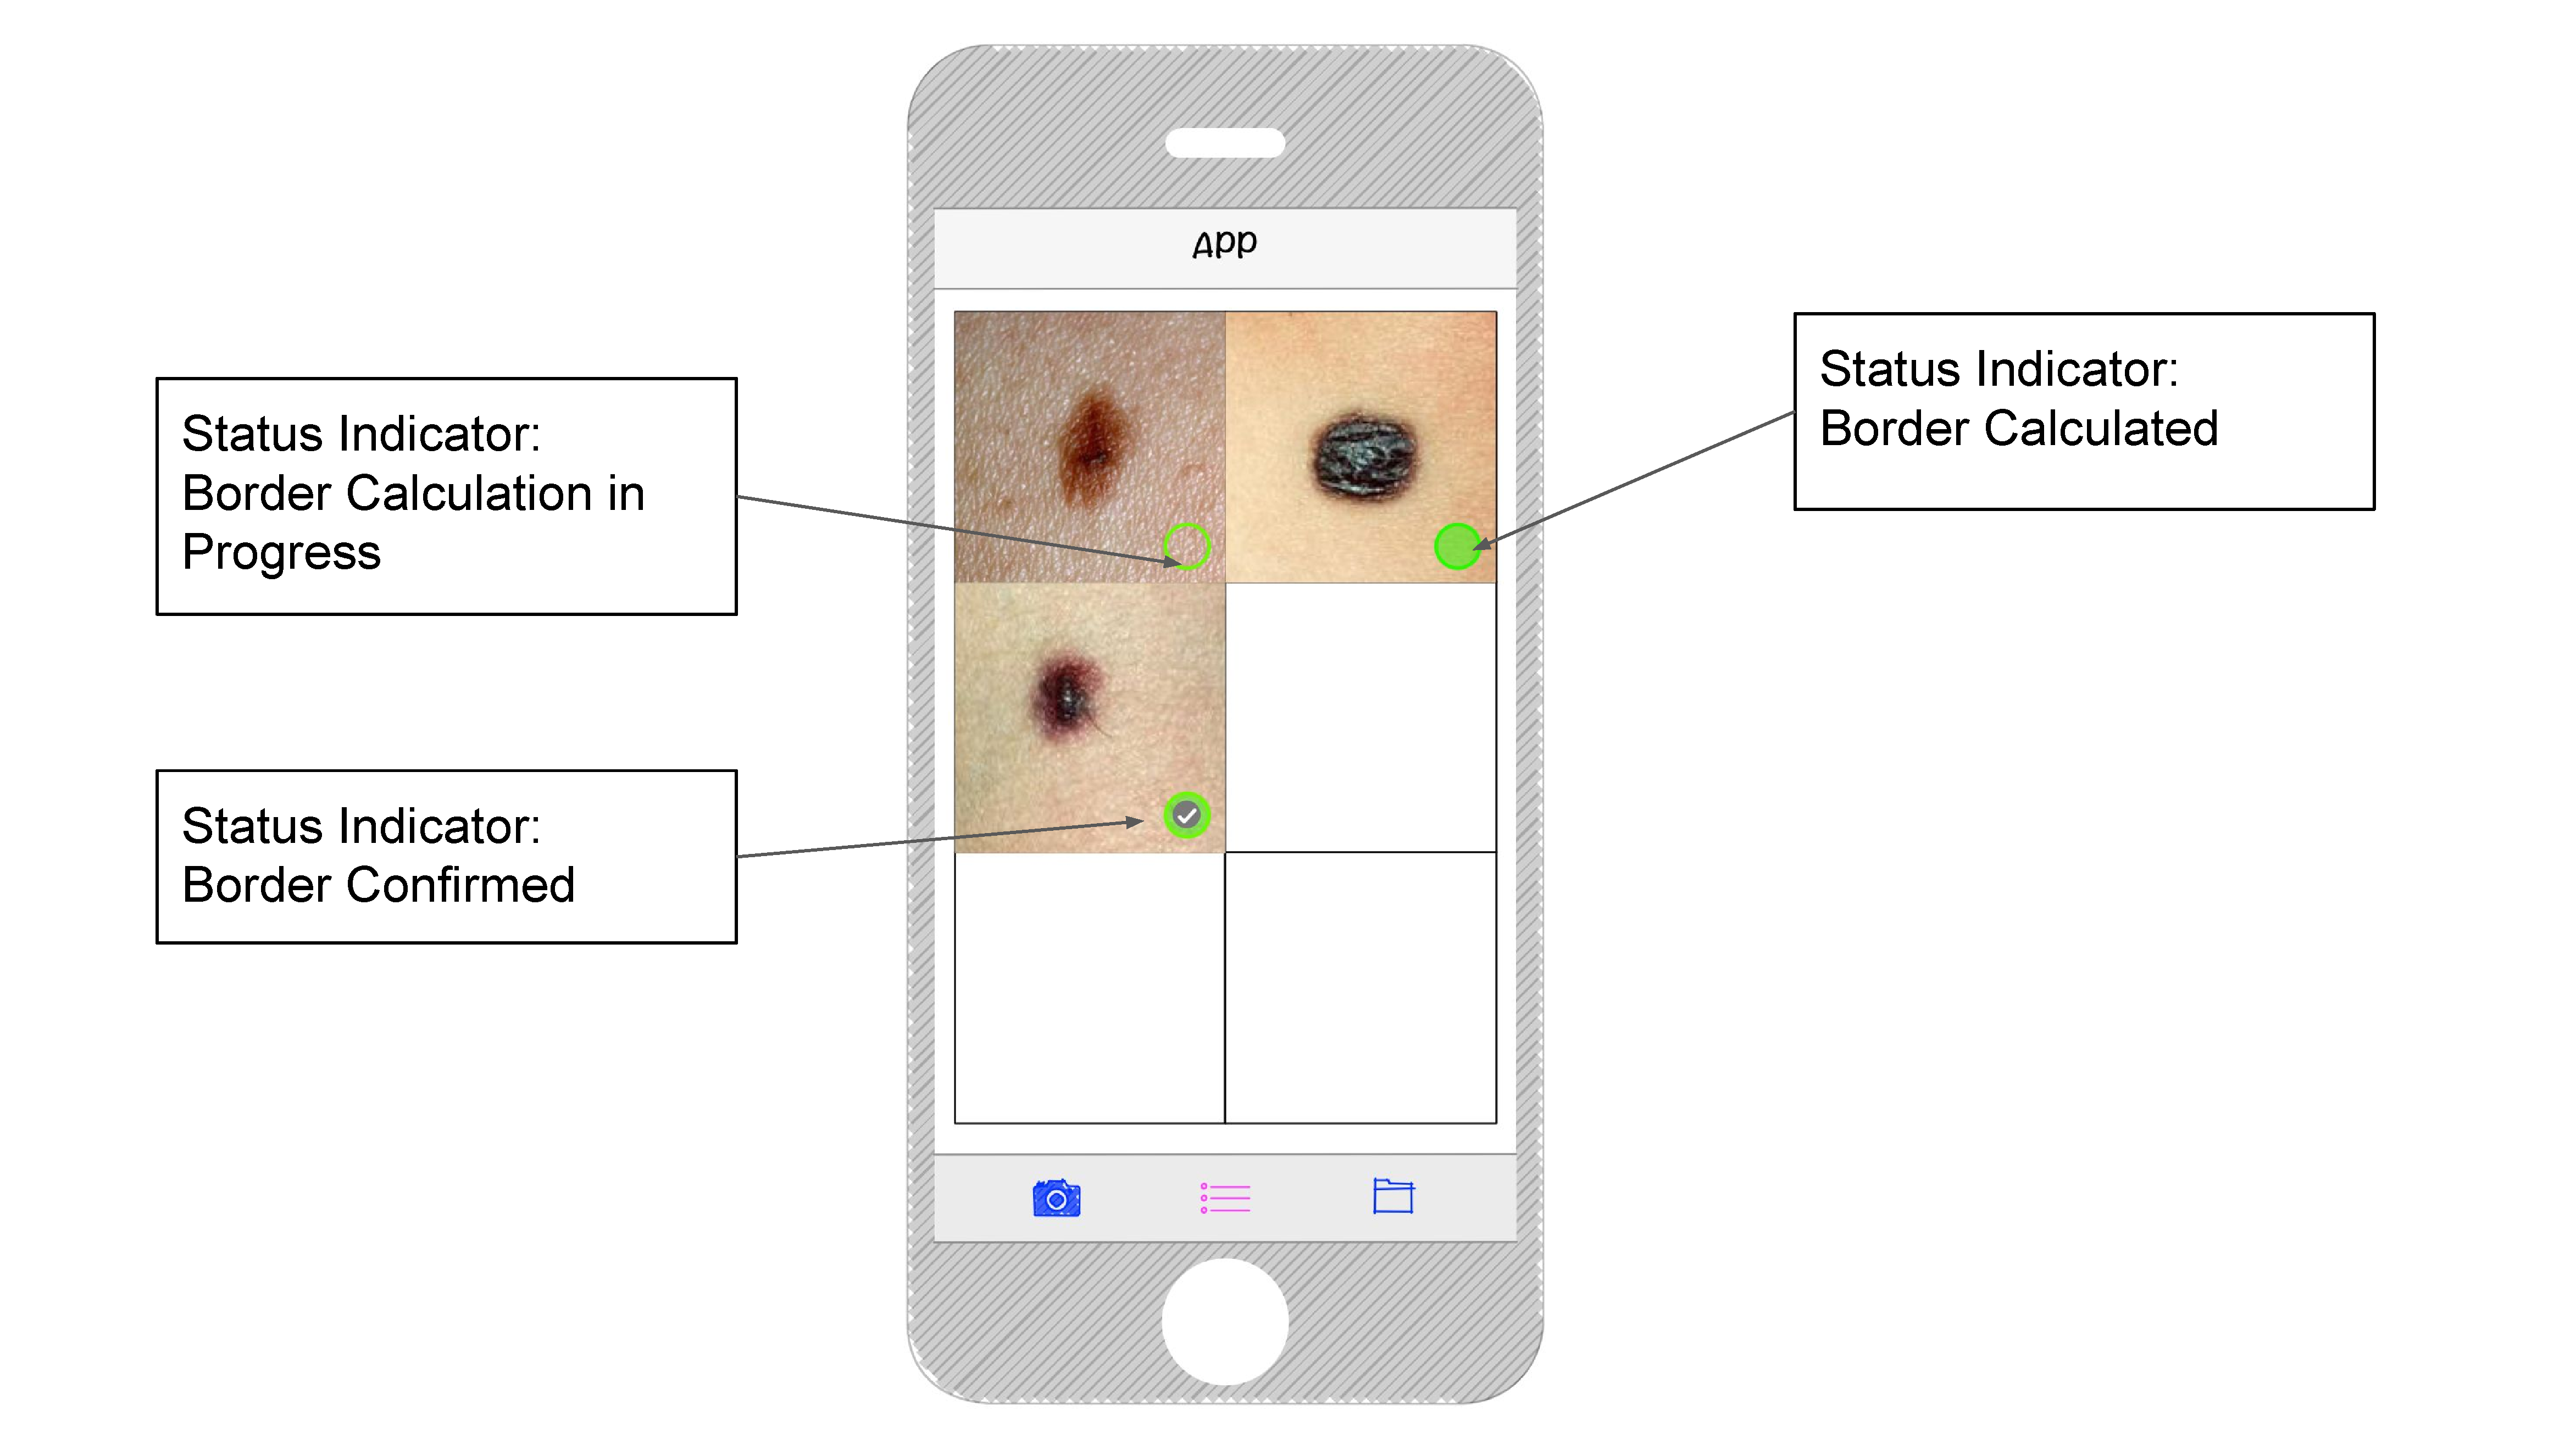
\includegraphics[height=10cm,keepaspectratio]{assets/GUI/image_list_view.pdf}
    \caption{Image List View}
    \label{fig:image_list_view}
\end{figure}

\begin{figure}[H]
    \centering
    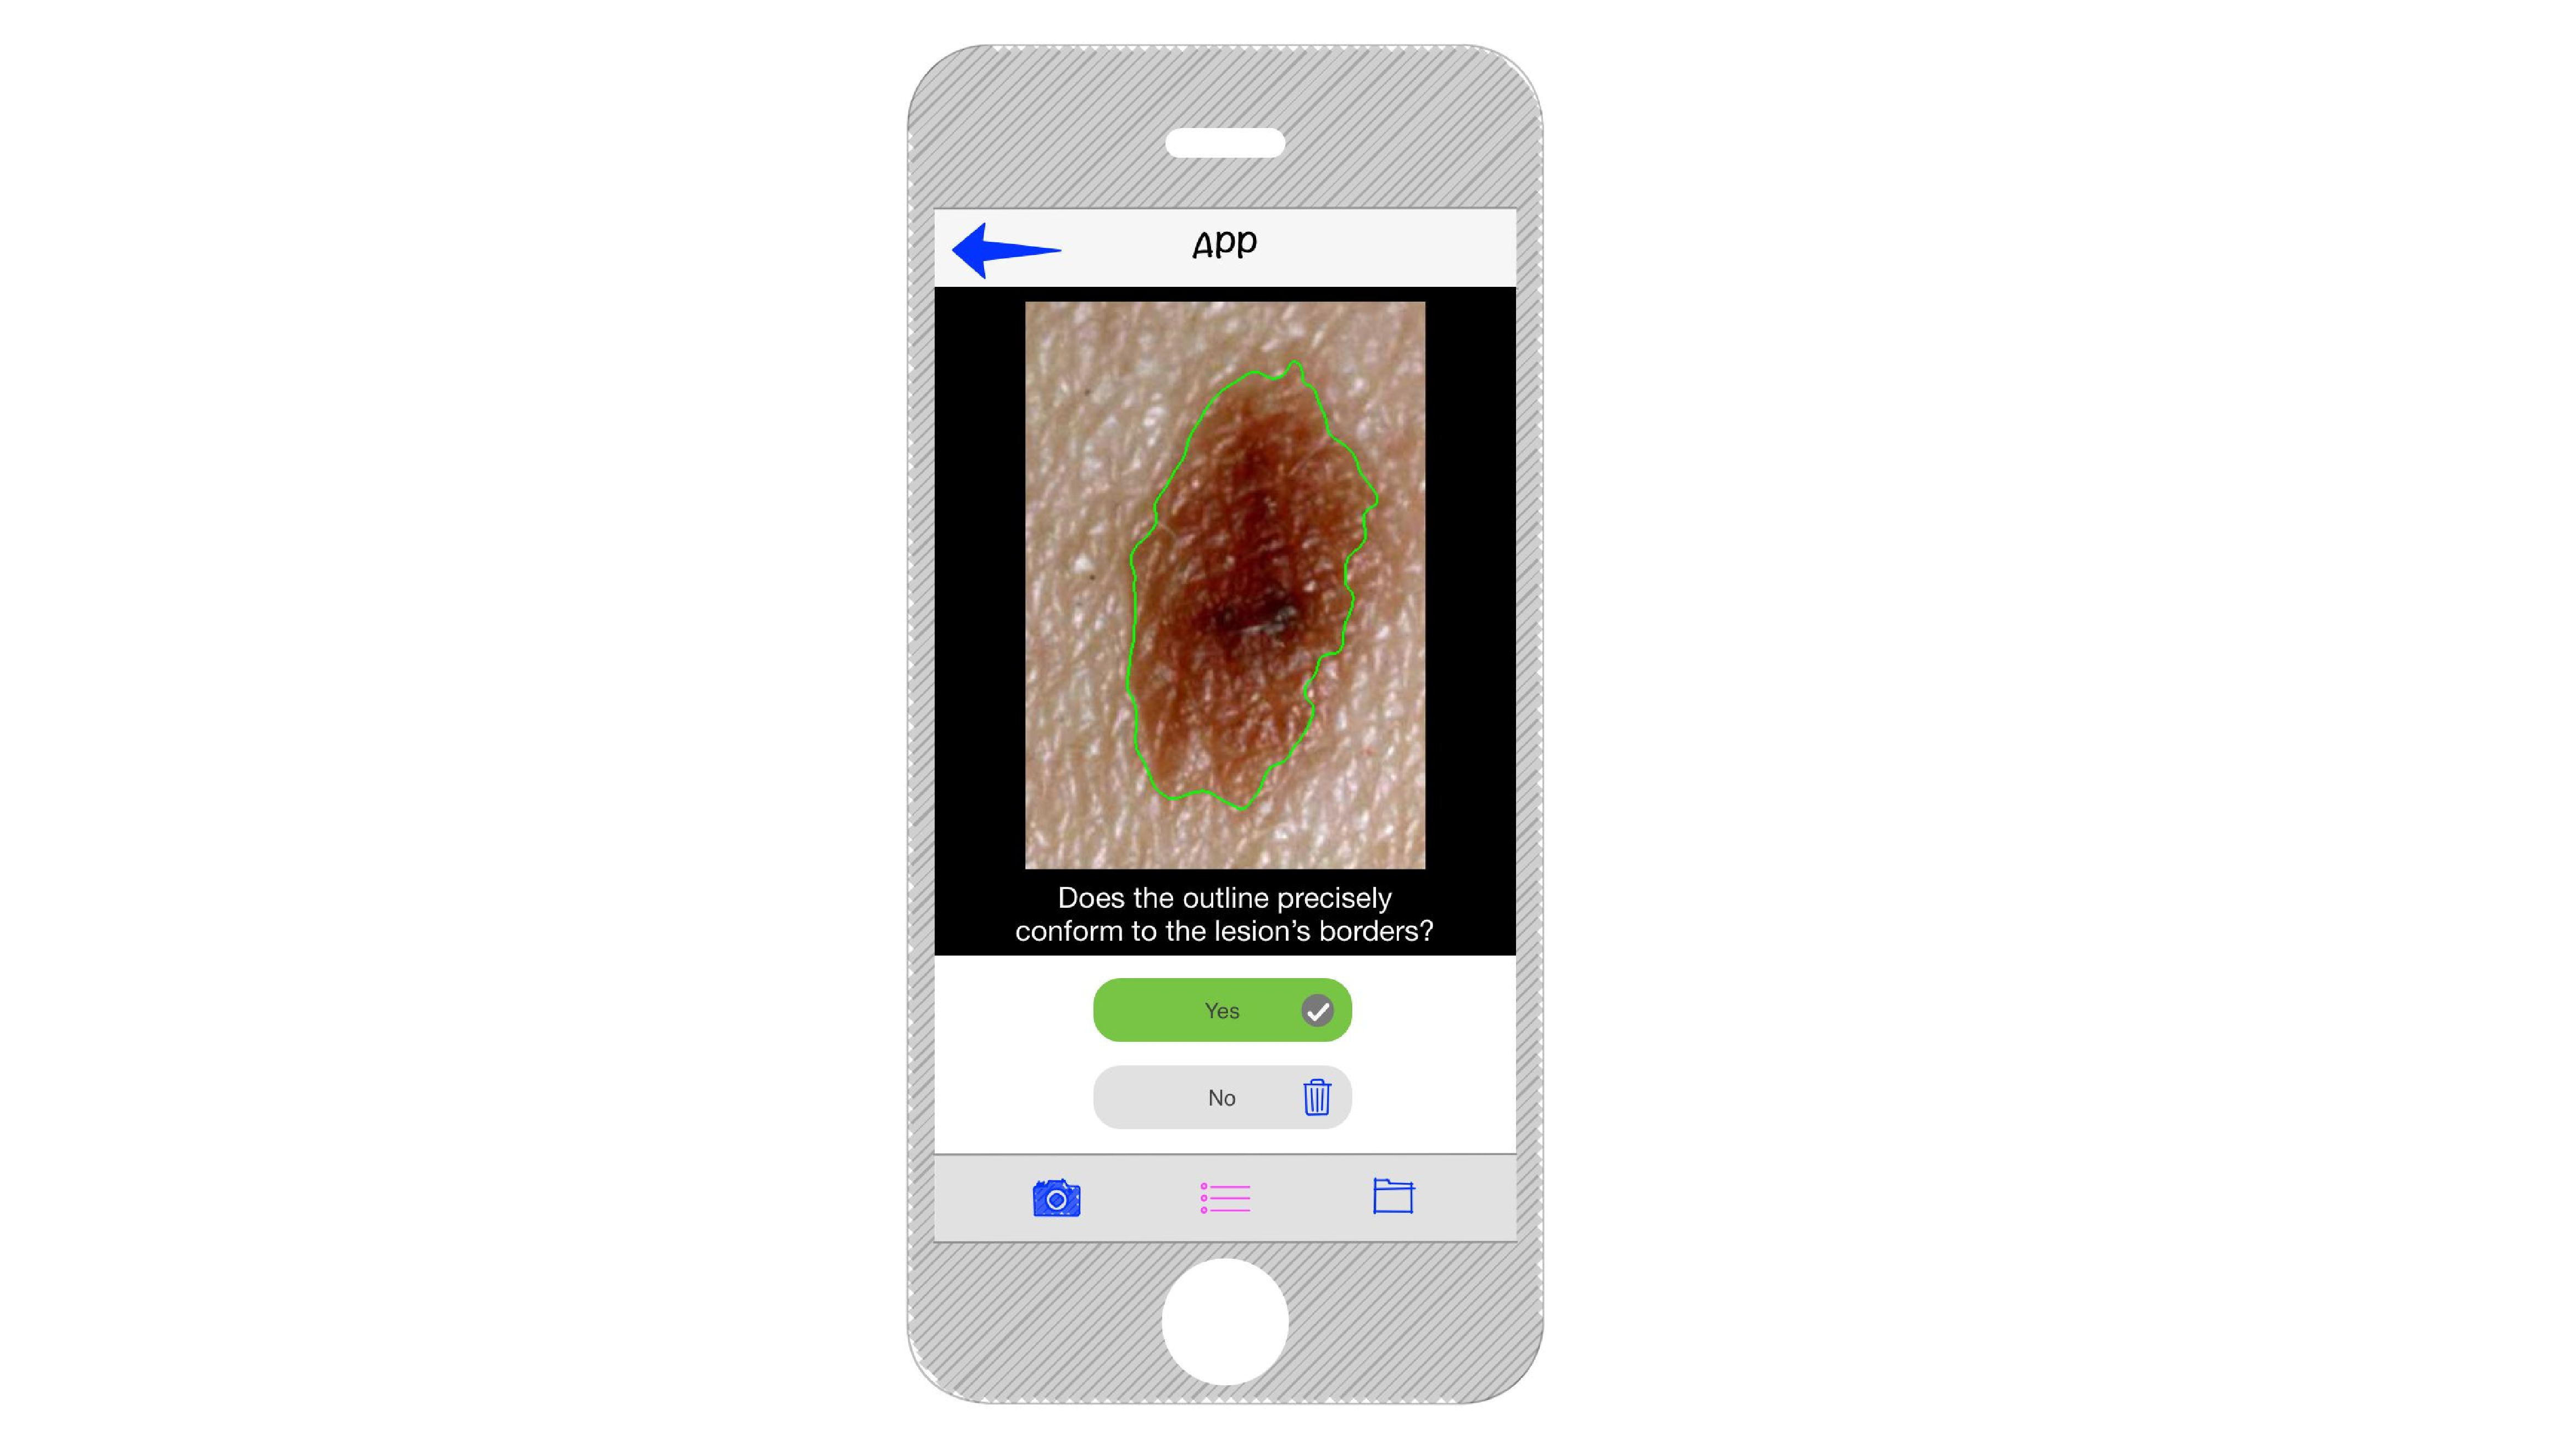
\includegraphics[height=10cm,keepaspectratio]{assets/GUI/border_confirm.pdf}
    \caption{Border Confirm View}
    \label{fig:border_confirm_view}
\end{figure}

\begin{figure}[H]
    \centering
    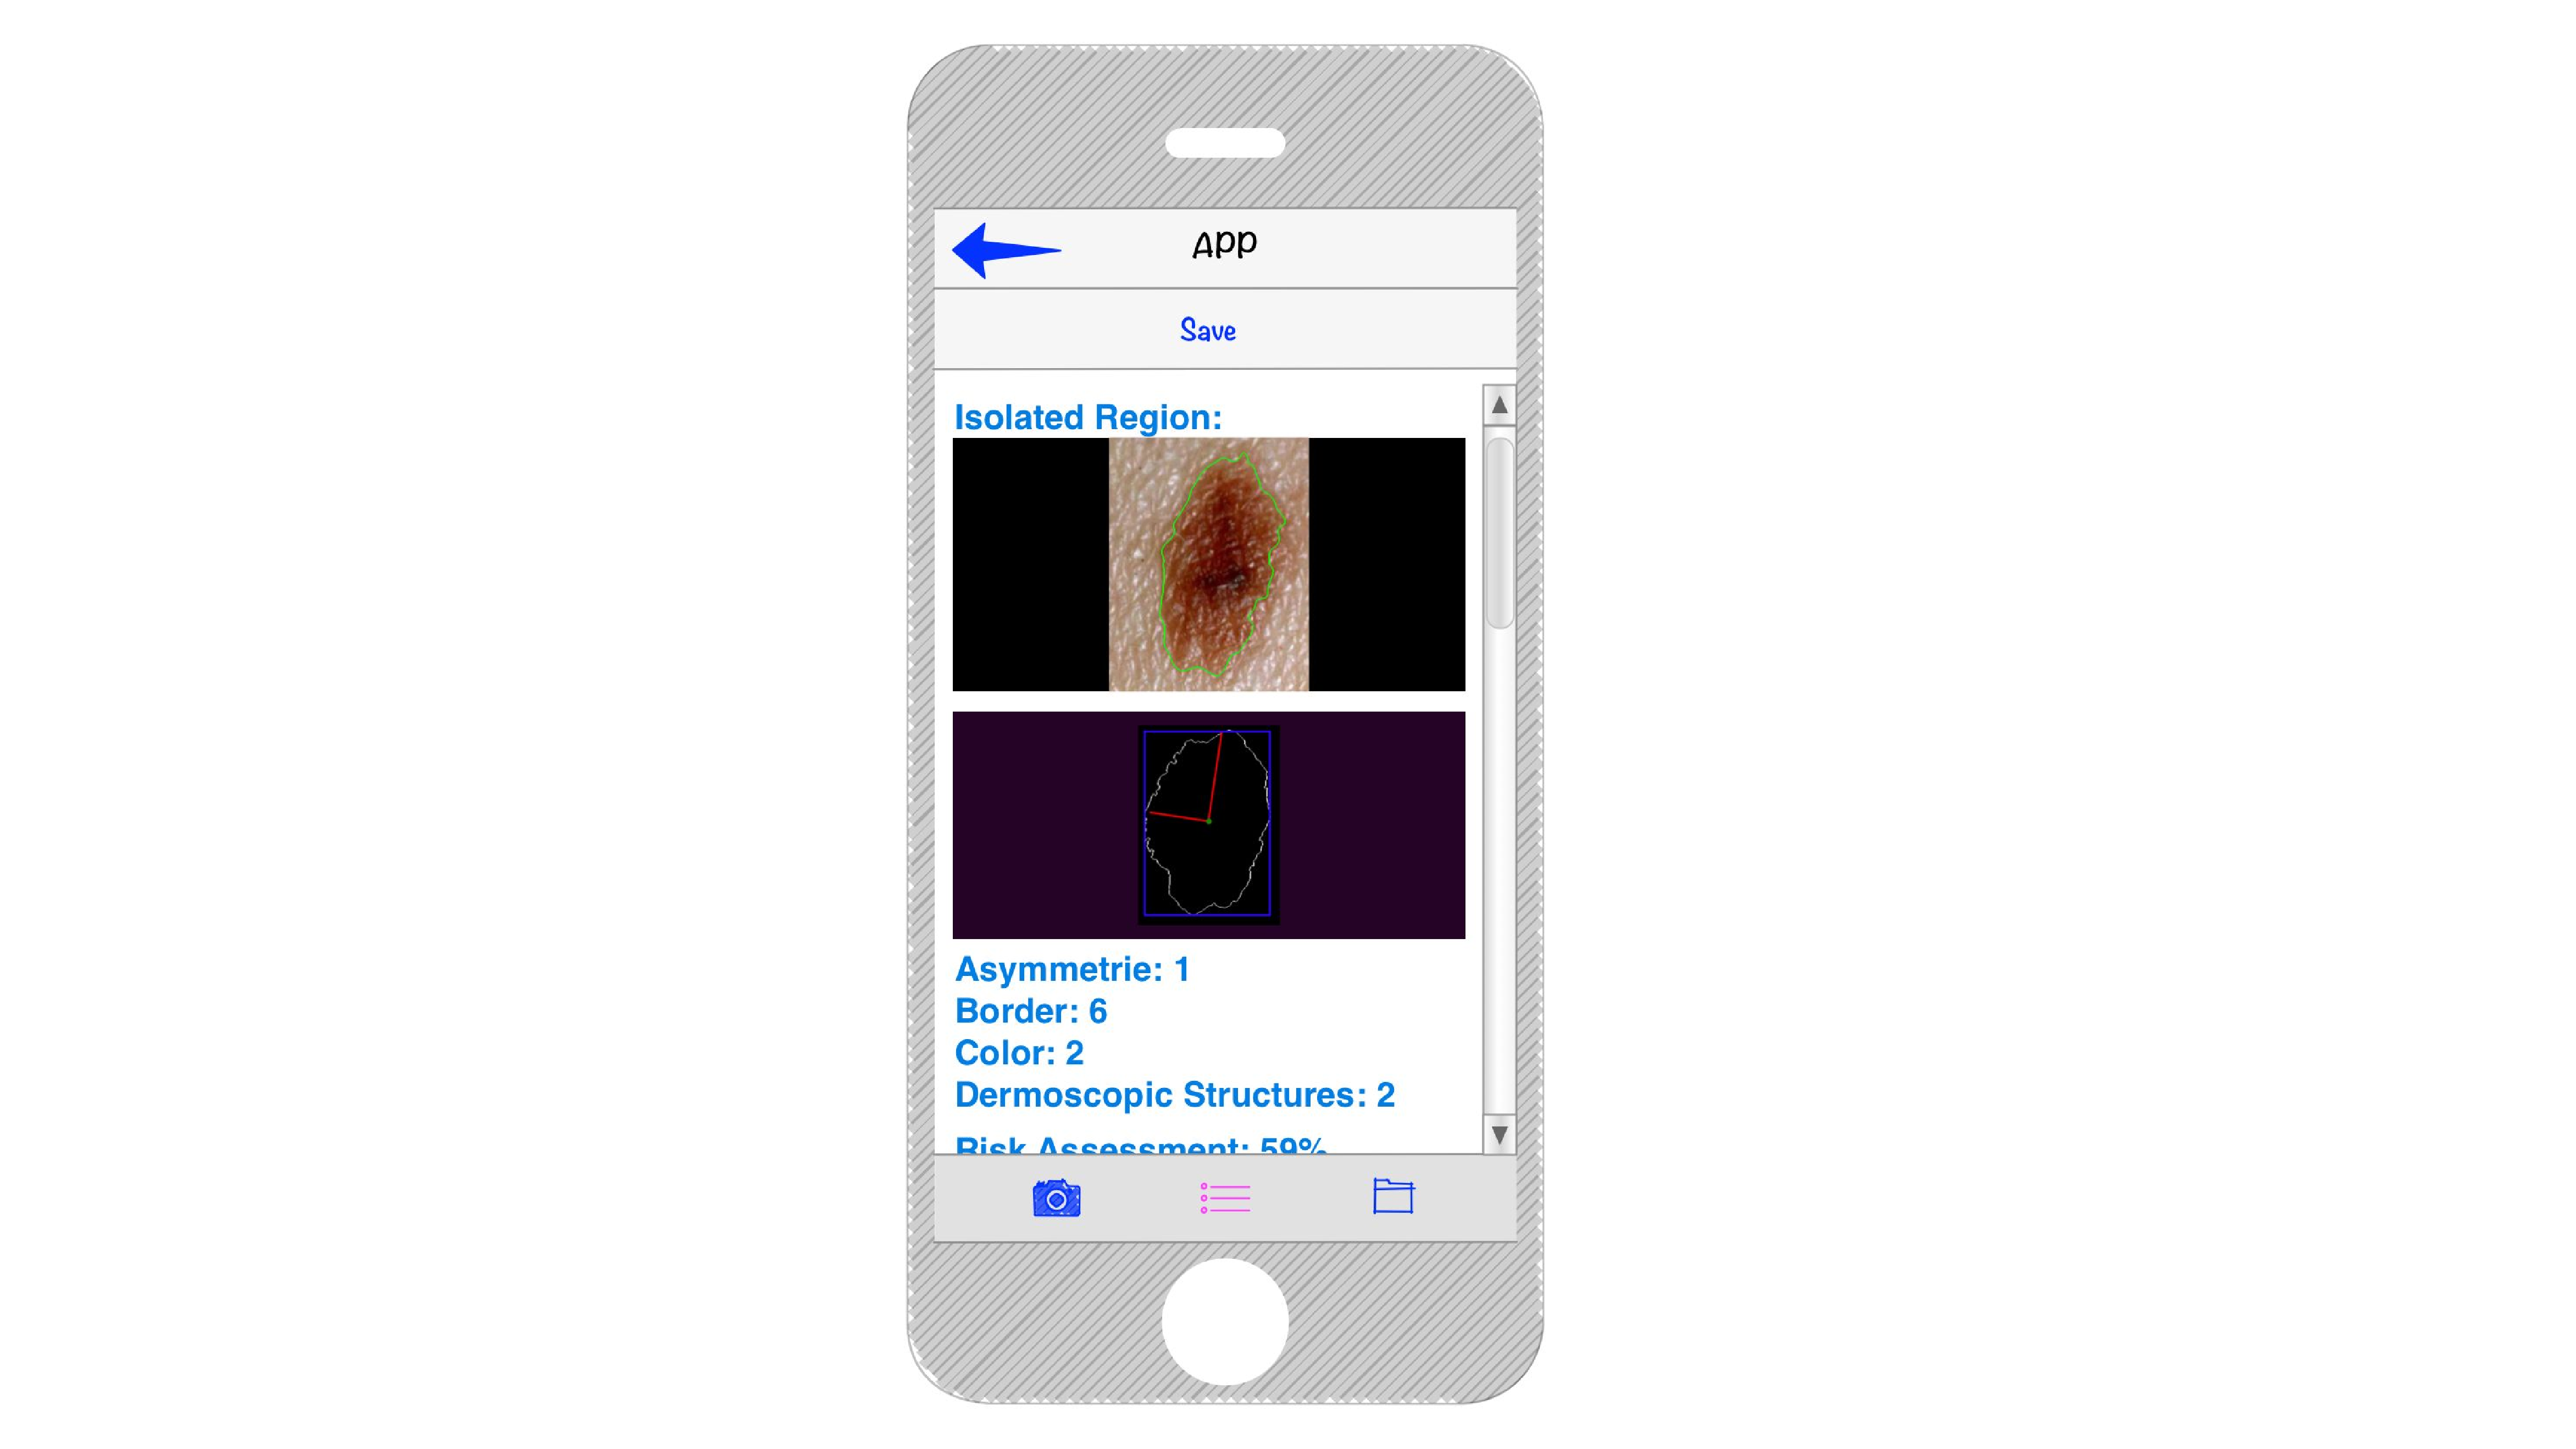
\includegraphics[height=10cm,keepaspectratio]{assets/GUI/image_detail_view.pdf}
    \caption{Image Detail View}
    \label{fig:image_detail_view}
\end{figure}

\begin{figure}[H]
    \centering
    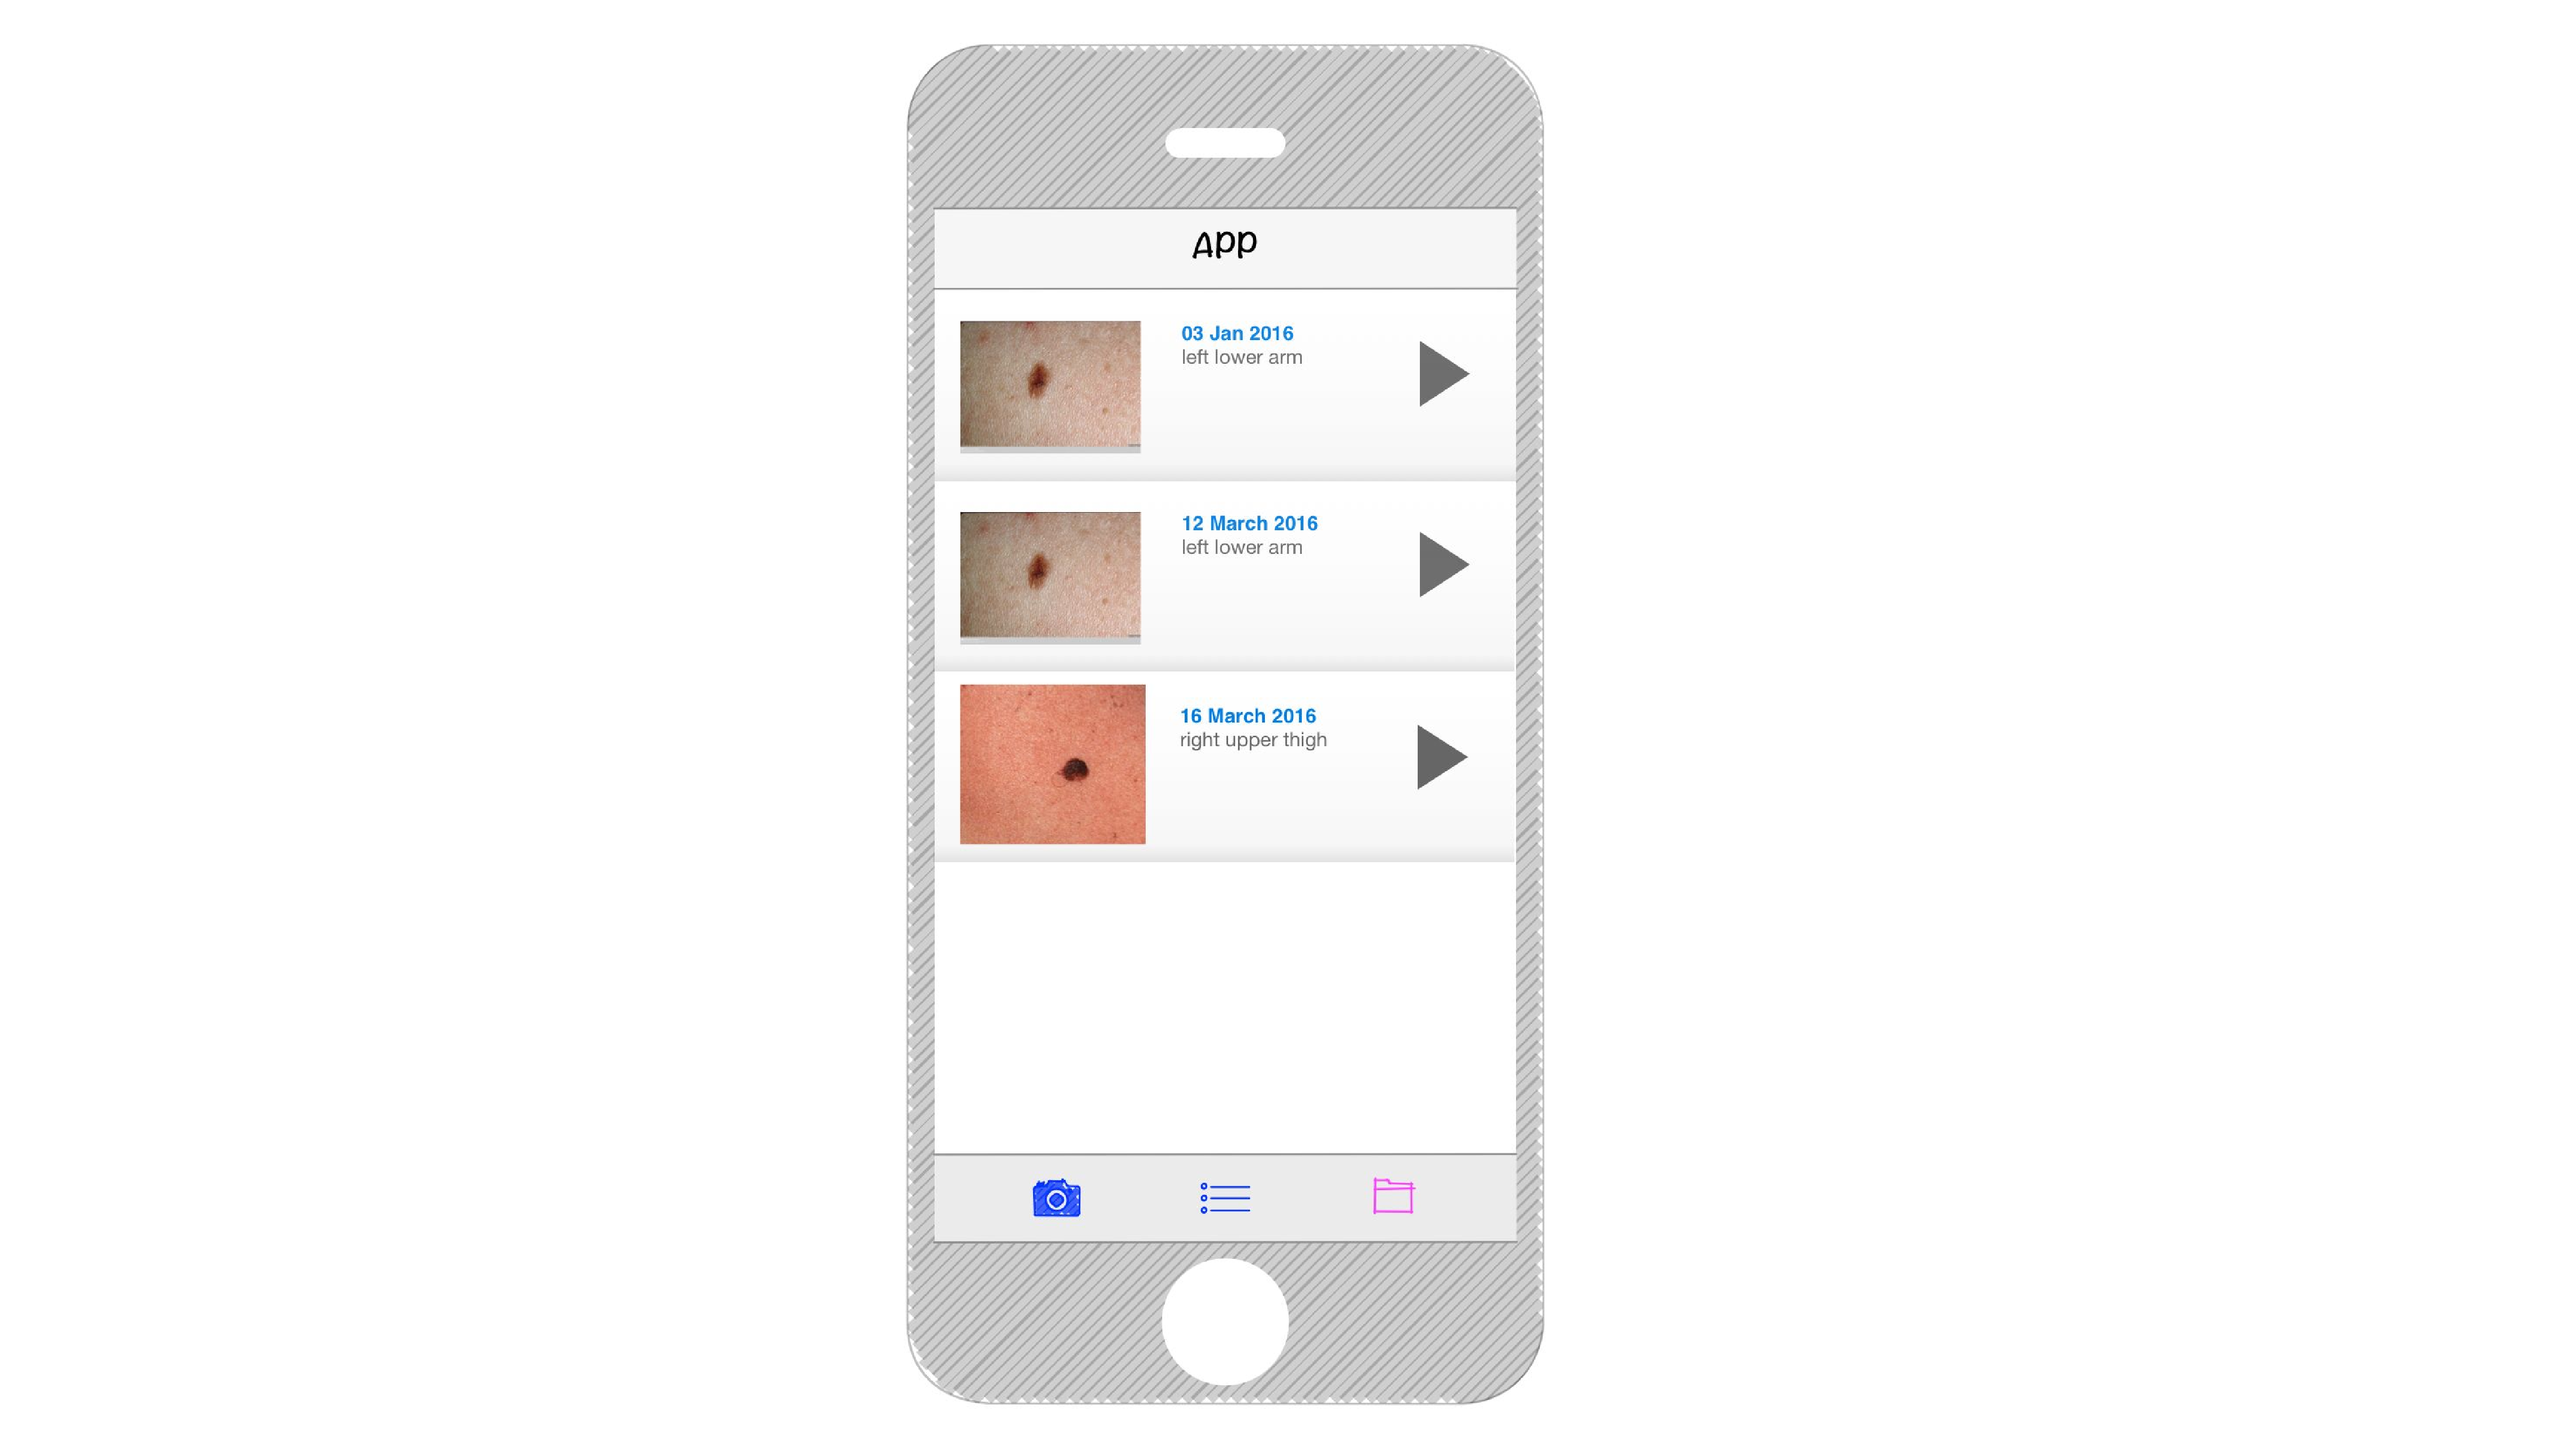
\includegraphics[height=10cm,keepaspectratio]{assets/GUI/archive_view.pdf}
    \caption{Archive View}
    \label{fig:archive_view}
\end{figure}

\begin{figure}[H]
    \centering
    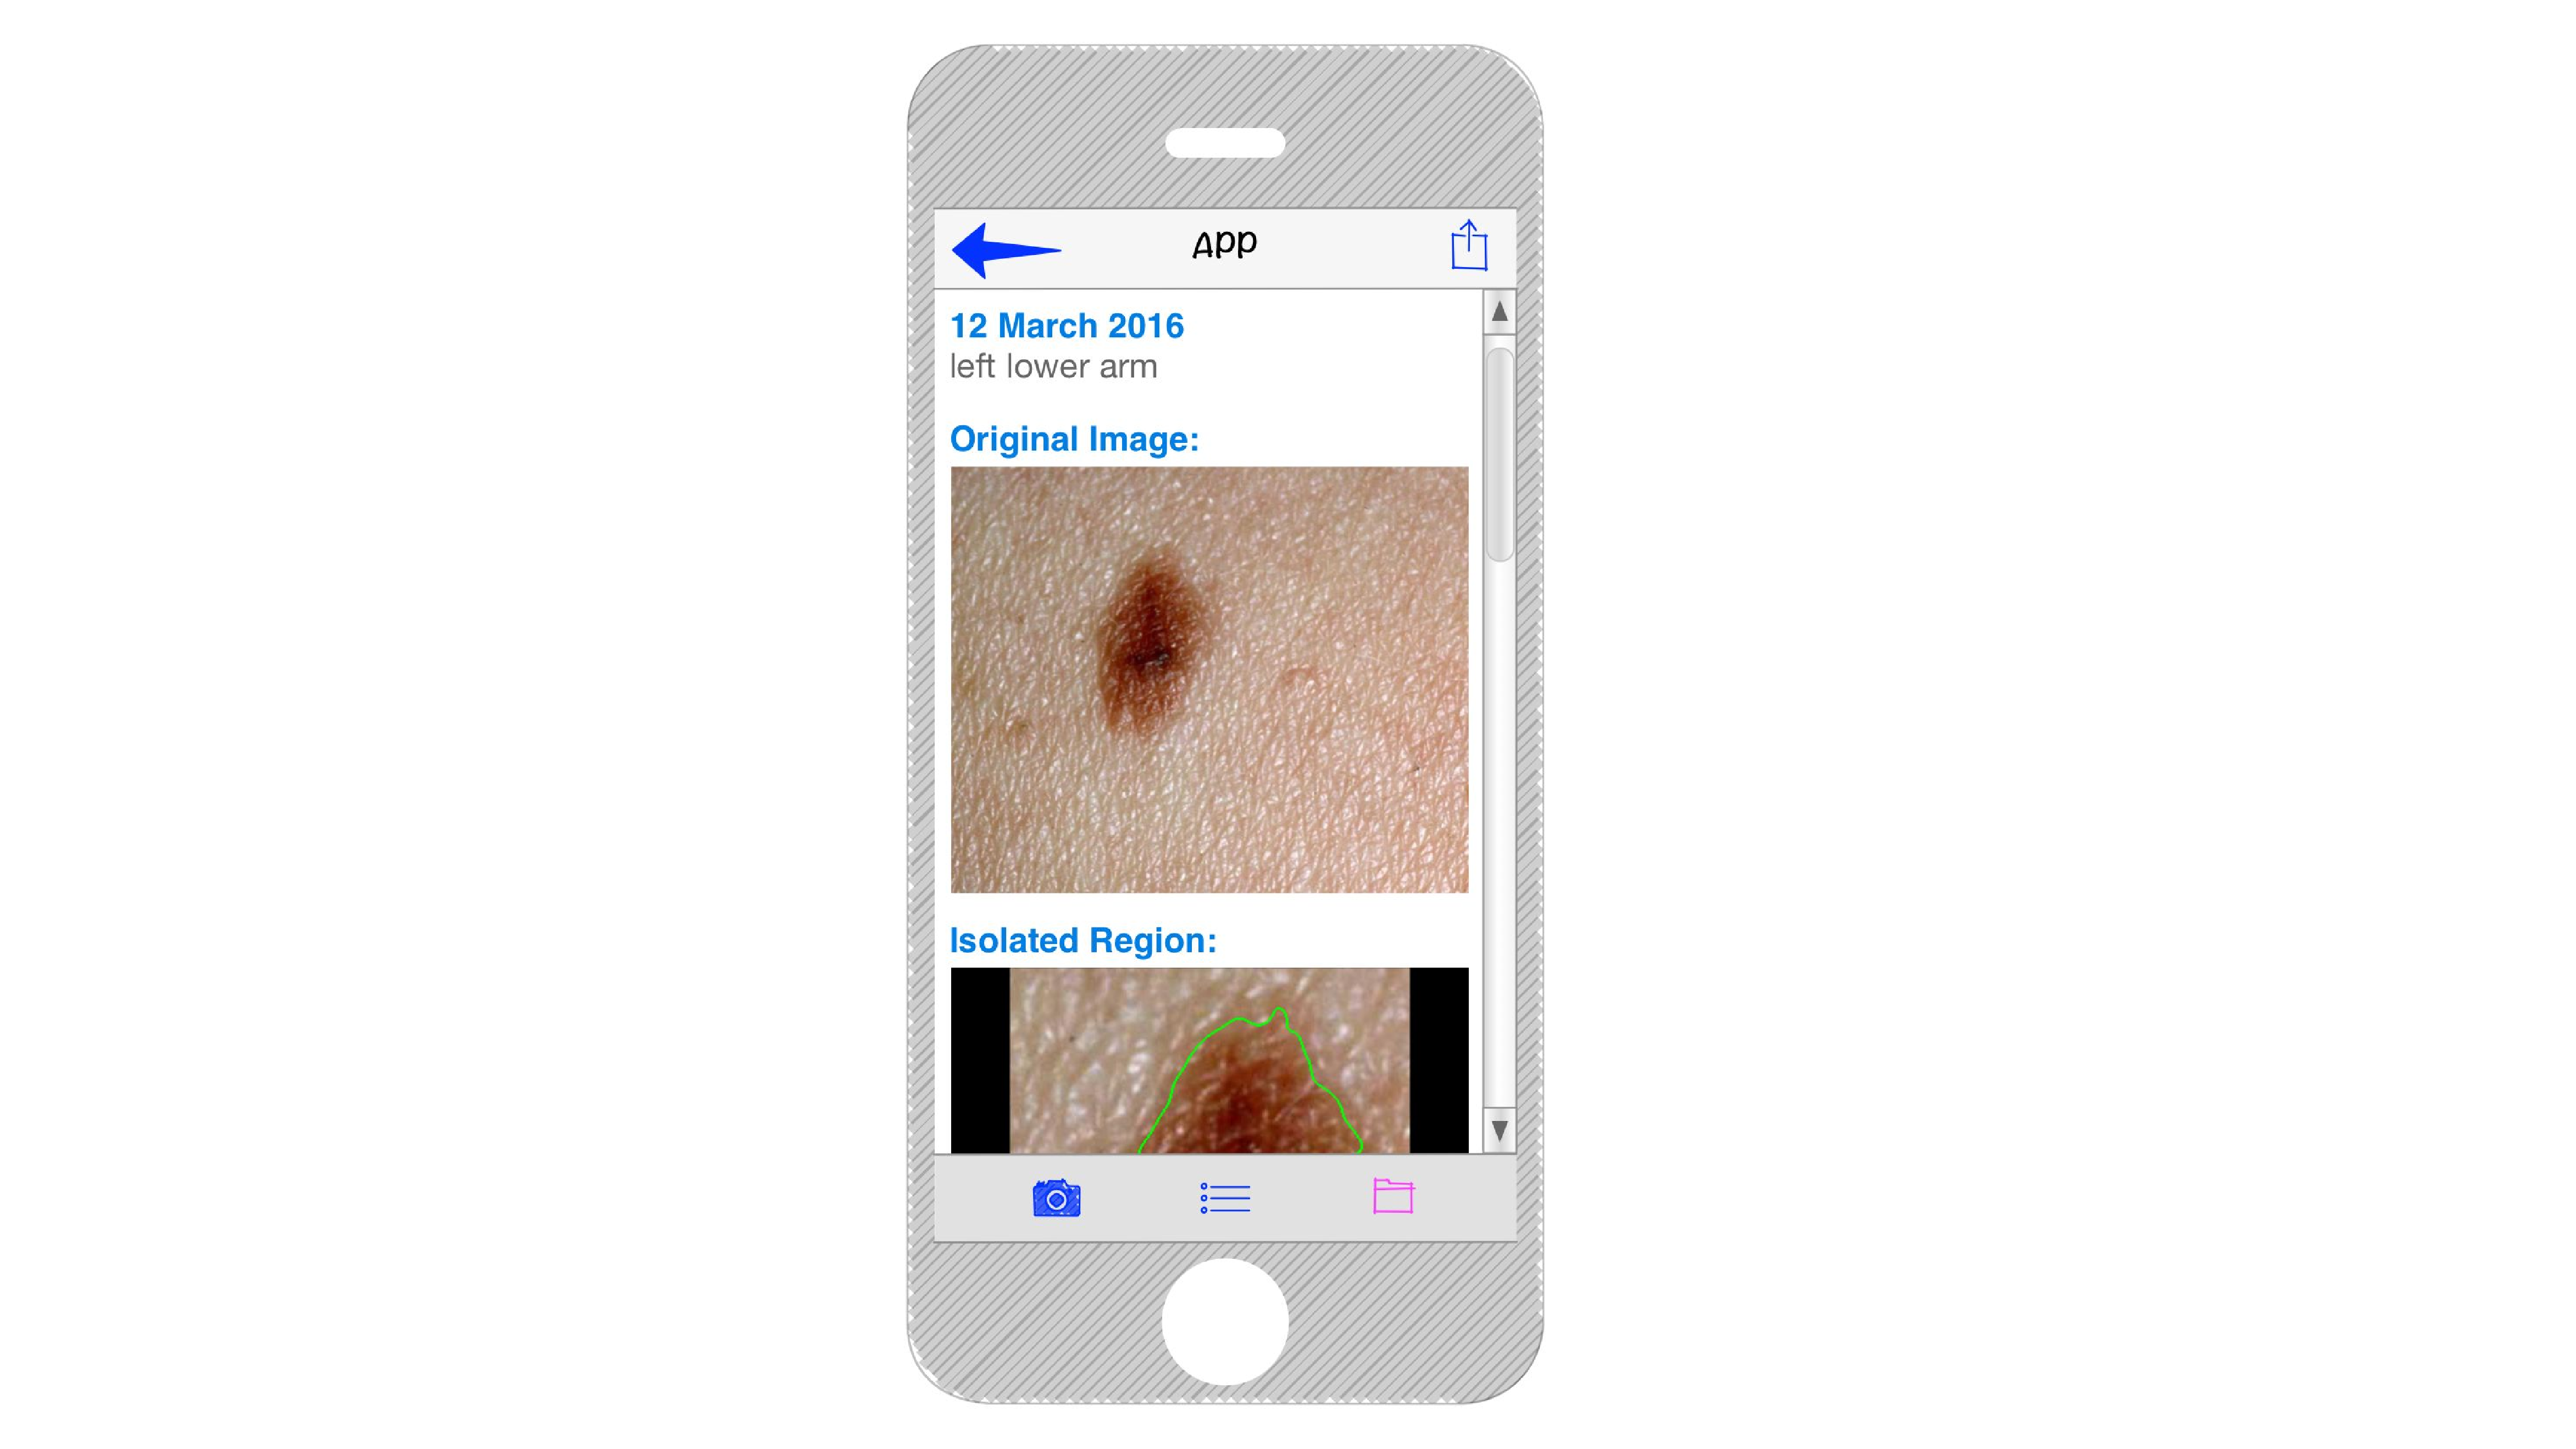
\includegraphics[height=10cm,keepaspectratio]{assets/GUI/archive_detail_view.pdf}
    \caption{Archive Detail View}
    \label{fig:archive_detail}
\end{figure}

\section{Data Structure}
\subsection{Server Data Structure}


\begin{figure}[H]
    \centering
    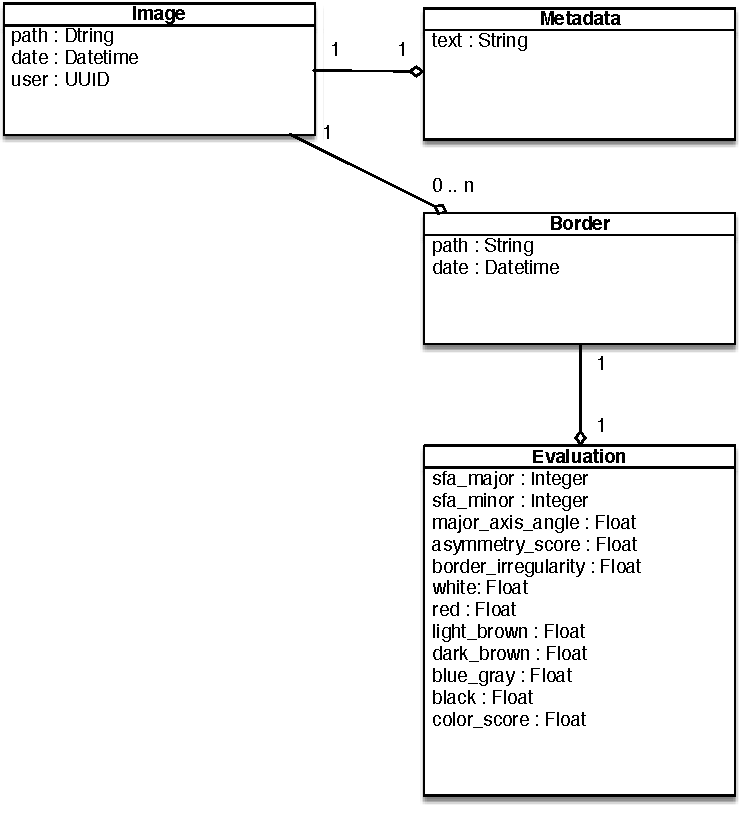
\includegraphics[height=8cm,keepaspectratio]{assets/data/server_data.pdf}
    \caption{Serverside Data Structure}
    \label{fig:data_server}
\end{figure}


\subsection{Client Data Structure}


\section{Software Architecture}
\subsection{MVC}
Since the 1970s the Model View Controller ( MVC ) pattern is the standard architectural design pattern for applications that present the user with a graphical user interface. It was developed out of a need for modularity, to encapsulate responsibility of specific concepts to separate program modules, or Separation of Concerns. MVC identifies three main components that program code should be grouped into, namely\cite{walther_2016}:

\begin{itemize}[label={}]

\item \textbf{Model}: The representation of some object of knowledge, encapsulates code managing the associated data and behaviour ( business-logic ).
\item \textbf{View}: The visual representation of the model. The view can feature or hide aspects of the model and thus act as a presentation filter. The view observe the model for changes and update the presentation accordingly.
\item \textbf{Controller}: The controller allows the user to interact with the model. It allows the user to trigger behaviours implemented in the Model.

\end{itemize}

In the classic MVC pattern the model does not "know" about the view or the controller. And the controller does not effect the view. Instead, both the view and controller monitor the model using an observer mechanism and synchronise themselves when updates to the model occur.

\begin{figure}[H]
    \centering
    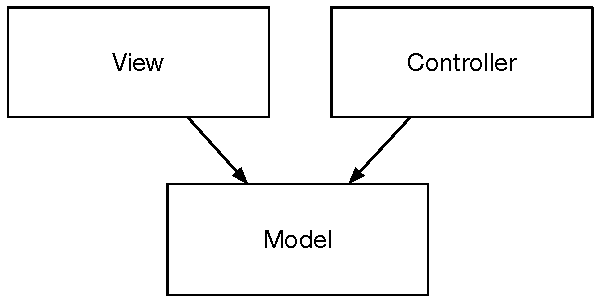
\includegraphics[height=6cm,keepaspectratio]{assets/concept/mvc_1.pdf}
    \caption{Classic MVC}
    \label{fig:mvc_1}
\end{figure}

\subsection{Modern MVC}

Modern MVC has evolved from being a software design pattern which handles components of an application to an architectural design pattern that defines the structure of an application itself. It has many similarities to the Layer Architecture. The responsibilities of each layer are slightly different to the typical presentation, business, and persistence layer definitions.

Most modern web frameworks such as Ruby on Rails, Symfony or the IOS environment refer to themselves as MVC based frameworks. The modern MVC concept has changed slightly. The component definitions are the same, but some responsibilities have shifted. Modern MVC strictly separates the model from the view. All modern frameworks state that the view should have as little logic as possible. Any logic implemented in the view should only be relevant to presentation. The view components should not directly reference the model components\cite{apple_MVC}\cite{symfony_MVC}.

\begin{figure}[H]
    \centering
    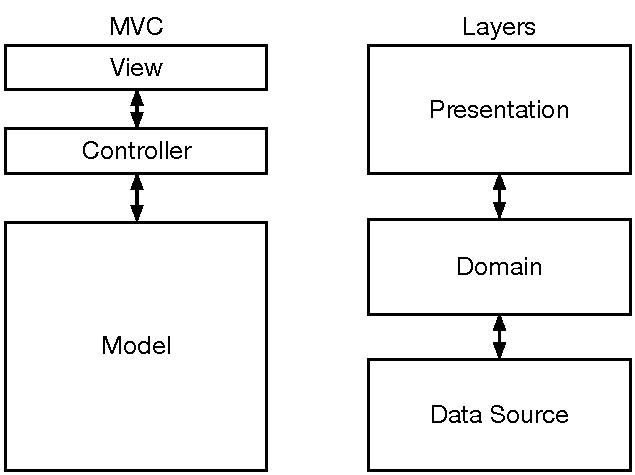
\includegraphics[height=6cm,keepaspectratio]{assets/concept/mvc_2.pdf}
    \caption{Modern MVC vs 3-Tier Layered Architecture}
    \label{fig:mvc_2}
\end{figure}

This division of responsibility has the added benefit of increased testability. GUIs are difficult to test, by removing as much logic as possible from the user interface there is less necessity to test it. The controller and model components can more easily be tested in isolation using normal unit tests\cite{mvp_testing}.

\subsection{MVC Derivatives}

Many MVC derivatives exist. The main differences are where the division of responsibility is made and how it is labeled. MVVM defines a view model instead of a controller. The view model acts as a facade around the model and introduces a data binder element that is responsible for keeping the view and view model synchronised. The MVT, calls the view a template and the controller a view. The slight difference is that the template is basically a static file, with no logic, and placeholders for the data. The Django web framework uses this model, but there is little difference to the other MVC derivatives such as MVP ( model view presenter ). The AngularJS web framework attempts to end the discussion of which design to follow by labelling itself a MVW ( Model View Whatever ) framework\cite{mvw}.


\begin{figure}[H]
    \centering
    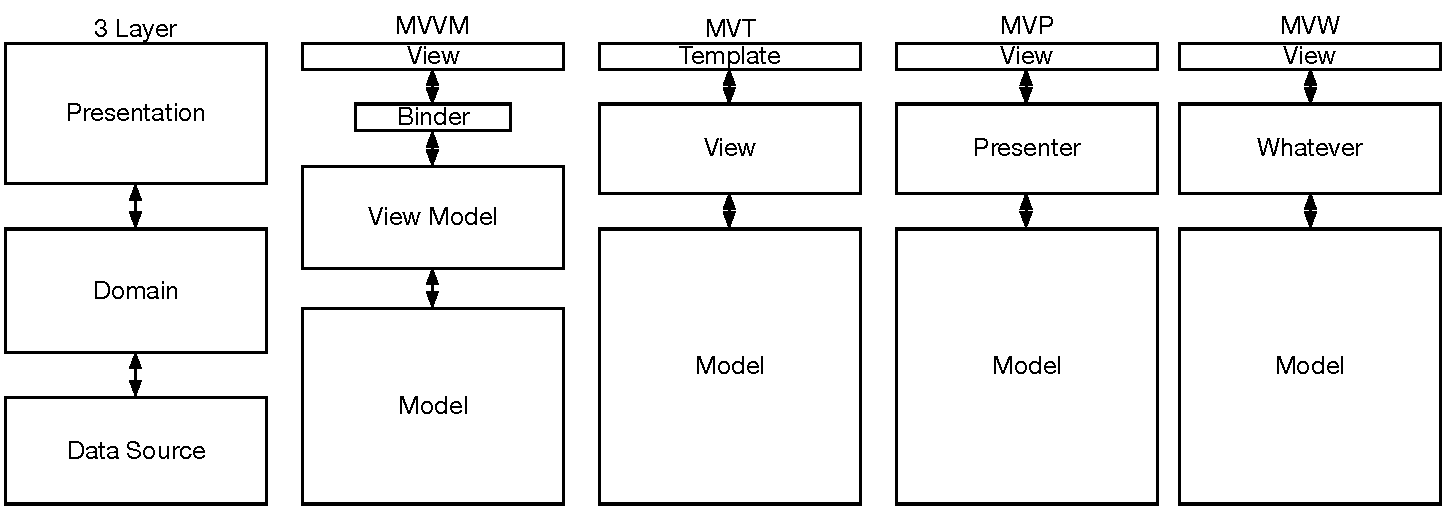
\includegraphics[height=6cm,keepaspectratio]{assets/concept/mvc_3.pdf}
    \caption{MVC Derivatives in relation to 3-Tier Layer}
    \label{fig:mvc_alt}
\end{figure}

\subsection{MVC and Smart Phone Applications}

Although most frameworks and environments targeted toward mobile application development use concepts from MVC, it can be difficult to define strict devision of responsibility, especially in conjunction with services provided from an online server. Often the responsibilities of the controller are reimplemented server side, some model management might occur in the app. Server and application code are developed using different languages and often most likely different developers. One solution is is to develop the app as a thin client, where it basically becomes the view component of MVC and the controllers and model are implemented on the server. Taken to the extreme, the app runs in a standard web browser and server provides the view components that emulate a native mobile user interface. This is referred to as a web app. Any logic in the view is implemented using javascript. Hardware support is limited to what the mobile browser provides access to. In order to extend hardware support a hybrid approach can be used in which the app implements a custom browser view which is extended with native capabilities. Here the division of responsibilities as defined by MVC become fuzzy. A fully native app working in conjunction with a web server will not conform well to the definitions of MVC.

\subsection{Considerations}

From the prioritised requirements defined above two important issues have an impact on architectural design decisions. Cross platform integration and extendability. The image processing and risk assessment algorithms are a complex combination of existing python based libraries and custom code. The rational behind choosing python as the basis is explained in detail in previous chapters. The disadvantage of choosing python for the basis of a mobile application is that is it not easily deployable on mobile hardware. Regardless of the decision to use python, the complexity of these algorithms would make it difficult and costly to implement in a cross platform manner in any language.

The solution is to offload the image processing and risk assessment algorithms to an online server running a python environment. The mobile application can interface with the online server in such a way that the process is transparent to the user.

The requirement for extendability and maintenance ( updatability ) becomes much easier as well. Updating the complex algorithms in multiple languages on multiple platforms and deploying updates to all existing users via the iTunes and Android shop platforms is not necessary. Instead only the server code needs to be updated. In the best case the phone-side app will not have to be updated at all.

Still the question remains, what architecture design pattern best covers the requirements of a mobile app with online server integration.

\subsection{VIPER}

VIPER is a new software architecture pattern which extends MVC with some addition concepts that make it more adaptable to mobile applications, especially when they are extended with online server based services. The classic controller is split into a presenter and a controller, the model component is split into a central data manager communicating with many services and entities\cite{viper}.

\begin{figure}[H]
    \centering
    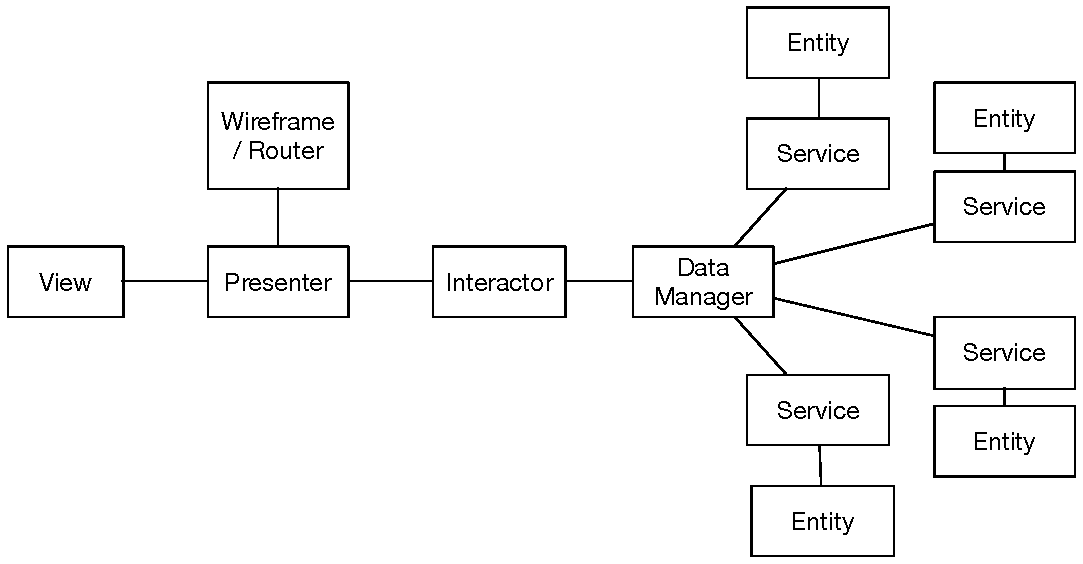
\includegraphics[height=7cm,keepaspectratio]{assets/concept/viper.pdf}
    \caption{VIPER Overview}
    \label{fig:viper}
\end{figure}

\begin{itemize}[label={}]

\item \textbf{View}: The view corresponds to the view as defined in modern MVC definitions, it is a slim component with as little logic as possible. It presents the current state of the models and provides “widgets” with which the user can interact.
\item \textbf{Presenter}: The presenter passes data to the view and handles events from the view. The presenter might perform some basic validation, in the case of a user sign-up scenario, for example, the presenter might validate that a user’s email is indeed formatted as a correct email, it will not validate if the email has already been used by someone else.

\item \textbf{Interactor}: Business logic is handled by the interactor. Most a what the model component in MVC was responsible for is handled here. The interactor however does not know anything about data storage, databases, or persistence. It does not know if data is local or accessible via a network.

\item \textbf{Data Manager}: To the Interactor the data manager looks like a database, with the difference that the it knows how to notify the interactor when data is available. The data manager will receive requests from the interactor, check it’s local cache, perform external service requests if necessary, then pass data back to the interactor once available.
\item \textbf{Service}: Services are encapsulated processes that can be online or local. The service knows how to fetch or store data, it might be a local sqlite database, or it can encapsulate the communication to an online database via a REST-API.

\item \textbf{Entity}: The representation of the actual data. As the entity get passed through the system it might be in the form of a database entry, a json object, or data object.

\item \textbf{Wireframe / Router}: The wireframe initialises all the other classes and handles the transitions to other views in the app. The wireframe handles the current “state” of the app and might implement a “history” allowing the user to transition back to a previous view with the associated other components and data.


\end{itemize}

\section{Mobile Development Strategies}
\subsection{Pure Native vs Hybrid Native vs Hybrid vs Web Apps}

The mobile app market is segmented into several platforms. Each platform has it’s own framework, API, and language specifications and requirements. Android apps are written in java and access the Android APIs, iOS apps in Objective-C or Swift and interface with the iOS frameworks. Android and iOS cover about 94\% of the worldwide mobile market \cite{mobile_market}. A developer must decide which platforms are priorities, and how might programming effort be consolidated across multiple platforms. Several strategies exist, and there are many tool kits and frameworks that can help accelerate development.

\begin{itemize}[label={}]

\item \textbf{Web Apps}: The simplest development strategy is to develop an HTML based web page that is disguised to appear and behave like a mobile app. The web app runs in a normal browser, is deployed from a standard web server. Model mobile web browsers offer javascript APIs that can access various other hardware components of the smart phone such as the compass, GPS/geolocation services, accelerometer, and the camera. Other services will remain inaccessible.

\item \textbf{Hybrid}: A similar strategy is to develop using javascript and html, but to package these elements into a “hollow” native app that is little else than a native view component with an embedded web browser. The web browser url is locked to the internal html files and appears to the user as a mobile app. though the user interface might slightly different that a pure native app. The advantage of a hybrid strategy is that the app can be distributed via the standard app stores increasing it’s marketability. It can also be extended with native components that might otherwise not be accessible to to a web app such as internal file storage and native data storage mechanisms.

\item \textbf{Pure Native}: The developer uses the development environment as provided by the phone manufacturer and has full access to all of the native hardware APIs, development kits and tools. The performance and responsiveness of a pure native app is much better compared to web and hybrid solutions. The user interface is built with the standard UI tools allowing a better user experience because the user is presented with familiar UI elements.

\item \textbf{Hybrid Native}: Recently several cross platform application frameworks have emerged that allow the developer to use a single language that can be compiled across several platforms. These frameworks unify the system and hardware APIs from different platforms into a single API. The limiting factor is how widely the unified API covers all the features the MDApp must integrate.

\end{itemize}



